%
% LaTeX template for the XLVII CILAMCE
% Paper: Comparison of MPM Integrators (USL, USF, MUSL) in Initial Accommodation vs. Abaqus
% ENGLISH VERSION (draft)
%
\documentclass[a4paper,10pt]{book}

% PACKAGES USED - packages that need to be previously installed on your computer
\usepackage[lmargin=2.5cm, rmargin=2.5cm, tmargin=2.5cm, bmargin=2.5cm ]{geometry}
\usepackage{graphicx}
\usepackage{times}
\usepackage{indentfirst}
\usepackage{fancyhdr}
\usepackage{titlesec}
\usepackage[english]{babel}
\usepackage[T1]{fontenc}
\usepackage{parskip}
\usepackage{setspace}
\usepackage{amsmath}

%%%%%%%%%%%%%%%%%%%%%%%%%%%%%%%%%%%%%%%%%%%%%%%%%%%%%%%%%%%%%%%%%
%%% My Additional Packages
%%%%%%%%%%%%%%%%%%%%%%%%%%%%%%%%%%%%%%%%%%%%%%%%%%%%%%%%%%%%%%%%%
\usepackage[utf8]{inputenc}
\usepackage{hyperref}
\usepackage{cleveref}
\usepackage{./pkg-crefNames} % <-- arquivo do template oficial, colocar na mesma pasta
\usepackage[labelsep=period]{caption}
\captionsetup{hypcap=false}

%BibTeX compatible with the CILAMCE format
\usepackage[numbers,sort&compress]{natbib}

\setlength{\bibsep}{0pt plus 0.3ex}
\renewcommand*{\bibfont}{\small}

\makeatletter
\renewcommand\bibsection
{
  \section*{References}
}

\renewenvironment{thebibliography}[1]
      {\section*{\refname}%
       \@mkboth{\MakeUppercase\refname}{\MakeUppercase\refname}%
       \list{\@biblabel{\@arabic\c@enumiv}}%
            {\settowidth\labelwidth{\@biblabel{#1}}%
             \leftmargin\labelwidth
             \advance\leftmargin-10pt
             \advance\leftmargin\labelsep
             \setlength\itemindent{10pt}
             \@openbib@code
             \usecounter{enumiv}%
             \let\p@enumiv\@empty
             \renewcommand\theenumiv{\@arabic\c@enumiv}}%
       \sloppy
       \clubpenalty4000
       \@clubpenalty \clubpenalty
       \widowpenalty4000%
       \sfcode`\.\@m}
      {\def\@noitemerr
        {\@latex@warning{Empty `thebibliography' environment}}%
       \endlist}
\renewcommand\newblock{\hskip .11em\@plus.33em\@minus.07em}
\makeatother
\bibliographystyle{./bib-cilamce} % <-- arquivo do template oficial, colocar na mesma pasta

%%%%%%%%%%%%%%%%%%%%%%%%%%%%%%%%%%%%%%%%%%%%%%%%%%%%%%%%%%%%%%%%%

% CONFIGURATION
\renewcommand*\arraystretch{1.5}
\renewcommand*\thesection{\arabic{section}}
\titleformat*{\section}{\large\bfseries}
\titleformat*{\subsection}{\bfseries}
\titlespacing\section{0pt}{20pt plus 2pt minus 2pt}{12pt plus 2pt minus 2pt}
\titlespacing\subsection{0pt}{20pt plus 0pt minus 0pt}{12pt plus 0pt minus 0pt}
\setlength{\parskip}{0pt}
\setlength{\parindent}{0.75cm}
\setlength\abovecaptionskip{6pt}

% --------------------------------------------------------------------------
% IMAGE PLACEHOLDER
% Use this command while final figures are not ready.
% Call it as: \imagemplaceholder{image description}{height}
% When the final image is ready, replace with \includegraphics.
% --------------------------------------------------------------------------
\newcommand{\imagemplaceholder}[2]{%
  \fbox{%
    \begin{minipage}[c][#2][c]{0.92\textwidth}
      \centering
      \textit{[INSERT IMAGE HERE:] #1}
    \end{minipage}%
  }%
}

% Smaller placeholder for side-by-side usage (two images per line)
\newcommand{\imagemplaceholdermeia}[2]{%
  \fbox{%
    \begin{minipage}[c][#2][c]{0.46\textwidth}
      \centering
      \textit{[INSERT IMAGE:] #1}
    \end{minipage}%
  }%
}

% --------------------------------------------------------------------------
% DO NOT EDIT - SPECIAL HEADINGS OF XLVII CILAMCE
% --------------------------------------------------------------------------
\fancypagestyle{first}
{
\fancyhf{}
\fancyfoot[RO]{\footnotesize \textit{CILAMCE-2026 \\
Proceedings of the XLVII Ibero-Latin-American Congress on Computational Methods in Engineering, ABMEC\\
Bogotá, Colombia, October 26-29, 2026}}
\renewcommand{\headrulewidth}{.0pt}
\renewcommand{\footrulewidth}{.5pt}
}

\pagestyle{fancy}
\fancyhf{}

\fancyfoot[LE]{\footnotesize \textit{CILAMCE-2026\\
Proceedings of the XLVII Ibero-Latin-American Congress on Computational Methods in Engineering, ABMEC\\
Bogotá, Colombia, October 26-29, 2026}}

\fancyfoot[RO]{\footnotesize \textit{CILAMCE-2026\\
Proceedings of the XLVII Ibero-Latin-American Congress on Computational Methods in Engineering, ABMEC\\
Bogotá, Colombia, October 26-29, 2026}}

\renewcommand{\headrulewidth}{.5pt}
\renewcommand{\footrulewidth}{.5pt}

% --------------------------------------------------------------------------
% EDIT: headers with short title and authors
% --------------------------------------------------------------------------
\fancyhead[LE]{\footnotesize \textit{Comparison of MPM integrators in initial accommodation}}
\fancyhead[RO]{\footnotesize \textit{Autor 1, Autor 2, Autor 3}}
% --------------------------------------------------------------------------

\begin{document}\thispagestyle{first}

% --------------------------------------------------------------------------
% DO NOT EDIT - LOGO OF XLVII CILAMCE
% --------------------------------------------------------------------------

\begin{figure}[ht!]
\vspace{-30pt}
\flushright

\includegraphics[width=6.69cm]{Figures/logo.png}
\end{figure}

% --------------------------------------------------------------------------
% PAPER TITLE
% --------------------------------------------------------------------------

\noindent
\textbf{\Large
Comparison of Material Point Method integrators (USL, USF and MUSL) in initial geostatic accommodation of a classical slope: an evaluation against Abaqus}
\vspace{18pt}

% --------------------------------------------------------------------------
% AUTHORS -- EDIT with real names, affiliations, and e-mails
% --------------------------------------------------------------------------

\noindent Evyllyn [Surname]$^1$, [Coauthor 2]$^1$, [Coauthor 3]$^1$

\vspace{18pt}

\noindent $^1$\textit{Laboratory for Scientific Computing and Visualization (LCCV), Federal University of Alagoas (UFAL)}

\noindent \textit{Maceio, Alagoas, Brazil}

\noindent \textit{email1@ufal.br, email2@ufal.br, email3@ufal.br}

\vspace{18pt}

% --------------------------------------------------------------------------
% ABSTRACT
% --------------------------------------------------------------------------

\noindent \textbf{Abstract.}
The Material Point Method (MPM) requires a quasi-static accommodation phase to establish the initial geostatic stress field before the main analysis. The quality of this accommodation depends directly on the time-integration scheme adopted, yet the literature on MPM accommodation has focused almost exclusively on dynamic-relaxation parameters, such as time step and damping, leaving the influence of the integrator itself largely unexamined. This work compares three widely used explicit MPM integrators -- Update Stress Last (USL), Update Stress First (USF) and Modified USL (MUSL) -- during the initial geostatic accommodation of a classical elastic slope with base of 60 m and height of 20 m. The reference solution is obtained from an implicit static FEM analysis in Abaqus. The comparison is carried out at an investigation point inside the slope, where the static Abaqus stress is contrasted with the temporal stress evolution computed by each MPM integrator until convergence. In addition to the local stress history, the study evaluates convergence through the decay of kinetic energy. The expected contribution is to clarify how the integration scheme affects the rate of accommodation, the oscillatory behavior of the response and the final agreement with the reference geostatic stress field.

\vspace{18pt}

\noindent \textbf{Keywords:} Material Point Method, time integrators, geostatic accommodation, USL, USF, MUSL.


% --------------------------------------------------------------------------
\section{Introduction}\label{sec:introducao}
% --------------------------------------------------------------------------

The Material Point Method (MPM) emerged as a hybrid development that combines particle-based Lagrangian ideas with the computational convenience of a fixed background mesh. The modern formulation introduced by \citet{Sulsky1994,Sulsky1995} made the method particularly attractive for problems with large deformations, complex stress history, and interface evolution, which are common features in geotechnical applications such as landslides, slope collapses, and progressive failure.

In brief, MPM represents the continuum through a set of material points carrying mass, velocity, stresses, strains, and internal variables. At each time step, this information is projected onto a background mesh, the nodal equations of motion are solved, and nodal quantities are interpolated back to the material points. This combination avoids the severe mesh distortion typical of purely Lagrangian methods while preserving the material description required for constitutive updates.

Before the main analysis, however, a consistent initial geostatic state must be built. In MPM, this is usually done through a quasi-static accommodation phase under gravity, during which the system dissipates spurious kinetic energy and approaches an equilibrium stress field. The quality of this initial state is critical: any residual oscillation or stress error introduced at this stage propagates into subsequent analysis stages.

The quality of this initial accommodation is influenced by the adopted time-integration scheme. The three most common explicit MPM integrators -- \emph{Update Stress Last} (USL), \emph{Update Stress First} (USF), and \emph{Modified USL} (MUSL) -- have different energy-conservation and numerical-dissipation characteristics, which can directly affect the accuracy of the stress state at the end of accommodation.

Despite this, the literature on MPM accommodation is still heavily focused on dynamic-relaxation parameters, such as time step ($\Delta t$) and damping coefficient, while the effect of integrator choice remains underexplored. In this work, the comparison among USL, USF, and MUSL is performed during the initial geostatic accommodation of a classical linear-elastic slope with a 60 m base and 20 m height. The reference is an implicit static FEM solution obtained with Abaqus, and the central comparison is based on the temporal evolution of stress at a selected investigation point within the slope mass.


% --------------------------------------------------------------------------
\section{State of the Art and Literature Gap}\label{sec:estadoarte}
% --------------------------------------------------------------------------

The original MPM formulation, based on the USL scheme, was introduced by \citet{Sulsky1994} and later extended by \citet{Sulsky1995} for solid mechanics problems. To reduce numerical oscillations associated with particle crossing between background-grid cells, \citet{Bardenhagen2004} proposed the \emph{Generalized Interpolation Material Point Method} (GIMP), which is now widely adopted in modern MPM implementations.

In the geotechnical context, \citet{Solowski2015} investigated numerical damping parameters and stability conditions for MPM applications, while \citet{Fern2019} presented a comprehensive review of common geostatic-accommodation practices in MPM, including recommendations for choosing $\Delta t$ and damping. More recent systematic reviews of MPM variants, including total and updated Lagrangian formulations, were presented by \citet{deVaucorbeil2020}. \citet{Zhang2016} discussed time-step control and CFL stability in explicit MPM implementations, and \citet{LlanoServa2016} proposed ramped gravity loading as an accommodation strategy for slopes.

Despite this relevant body of contributions, none of the reviewed studies systematically addresses:

\begin{itemize}
    \item comparison among USL, USF, and MUSL specifically during the geostatic accommodation phase;
    \item validation of the post-accommodation MPM stress field against an implicit FEM reference solution (Abaqus);
    \item the effect of integrator choice on stress and kinetic-energy oscillations throughout accommodation;
    \item use of a kinetic-energy criterion as an objective and automated alternative to the traditional fixed-time criterion;
    \item a practical recommendation on which integrator converges faster to the correct geostatic state.
\end{itemize}

This work directly addresses these gaps, with specific focus on integrator choice during initial MPM accommodation.

% --------------------------------------------------------------------------
\section{MPM Integrators: USL, USF, and MUSL}\label{sec:integradores}
% --------------------------------------------------------------------------

The three explicit time-integration schemes considered in this work differ mainly in the order in which stress is updated relative to particle position and velocity updates. In all of them, the basic cycle includes: (i) projection of particle mass, momentum, and forces to the background mesh; (ii) solution of the nodal equations of motion; (iii) transfer of nodal velocities and accelerations back to particles; and (iv) kinematic and constitutive update of material points. What changes from one integrator to another is the exact stage where velocity gradient, incremental strain, and stress state are computed.

This apparently subtle difference affects numerical dissipation, transient response, and the rate at which the solution approaches geostatic equilibrium. Since the objective here is to compare temporal stress curves up to convergence, it is important to make these operational differences explicit rather than only naming the schemes.

% --------------------------------------------------------------------------
\subsection{USL -- Update Stress Last}\label{subsec:usl}
% --------------------------------------------------------------------------

In the USL scheme, stresses are updated last, after the particle kinematic update. In practical terms, the algorithm projects particle state onto the mesh, solves nodal equilibrium, updates velocities and positions, and only then computes incremental strains and stresses. For internal-force calculation in the current step, this strategy uses a stress state still linked to the previous step.

As a consequence, USL tends to produce a more oscillatory response during accommodation, especially when gravity is applied from the beginning and the system needs to dissipate initial energy quickly. On the other hand, the algorithm is simple, widely used, and naturally serves as a reference because it is tied to the classical MPM formulation.

% --------------------------------------------------------------------------
\subsection{USF -- Update Stress First}\label{subsec:usf}
% --------------------------------------------------------------------------

In the USF scheme, stress is updated before the final particle-position update. This means that velocity gradient and incremental strain are used earlier within the step, allowing internal-force calculation to already incorporate a more up-to-date stress state.

In geostatic-accommodation problems, this characteristic tends to reduce part of the lag observed in USL between kinematic and constitutive response. However, changing the algorithmic sequence also alters the balance between dissipation and oscillation propagation, so improved stability does not always automatically translate into closer agreement with the static reference solution.

% --------------------------------------------------------------------------
\subsection{MUSL -- Modified USL}\label{subsec:musl}
% --------------------------------------------------------------------------

The MUSL scheme introduces a double velocity update. After the first node-to-particle transfer, updated particle velocities are projected back to nodes, producing an intermediate correction before the final strain and stress computation. In other words, MUSL seeks better compatibility between particle kinematics and the nodal field within the same time step.

This second update usually improves mapping consistency and reduces numerical artifacts associated with particle-mesh-particle transfer, which is particularly relevant in simulations with large deformations or long accommodation periods. For this reason, MUSL is often considered a promising candidate for reproducing the reference geostatic state more stably, although this hypothesis still needs quantitative verification for the present problem.

% --------------------------------------------------------------------------
\section{Methodology}\label{sec:metodologia}
% --------------------------------------------------------------------------

% --------------------------------------------------------------------------
\subsection{Reference Model}\label{subsec:modelo_referencia}
% --------------------------------------------------------------------------

As the reference problem, a two-dimensional classical slope under linear-elastic behavior was adopted, with a 60 m base and 20 m height, subjected only to self-weight. This case represents an advance relative to simplified one-dimensional tests because it preserves interpretive clarity while introducing a spatially nontrivial stress field that is closer to real geotechnical applications.

The reference solution was obtained in Abaqus using a static analysis with gravitational loading, representing the target geostatic state. In MPM, the same domain is initially relaxed from a stress-free condition, allowing observation of how each integrator drives temporal evolution up to accommodation. The objective is not only to compare the final state, but also to evaluate the convergence path followed by each scheme.

\vspace{8pt}
\begin{center}
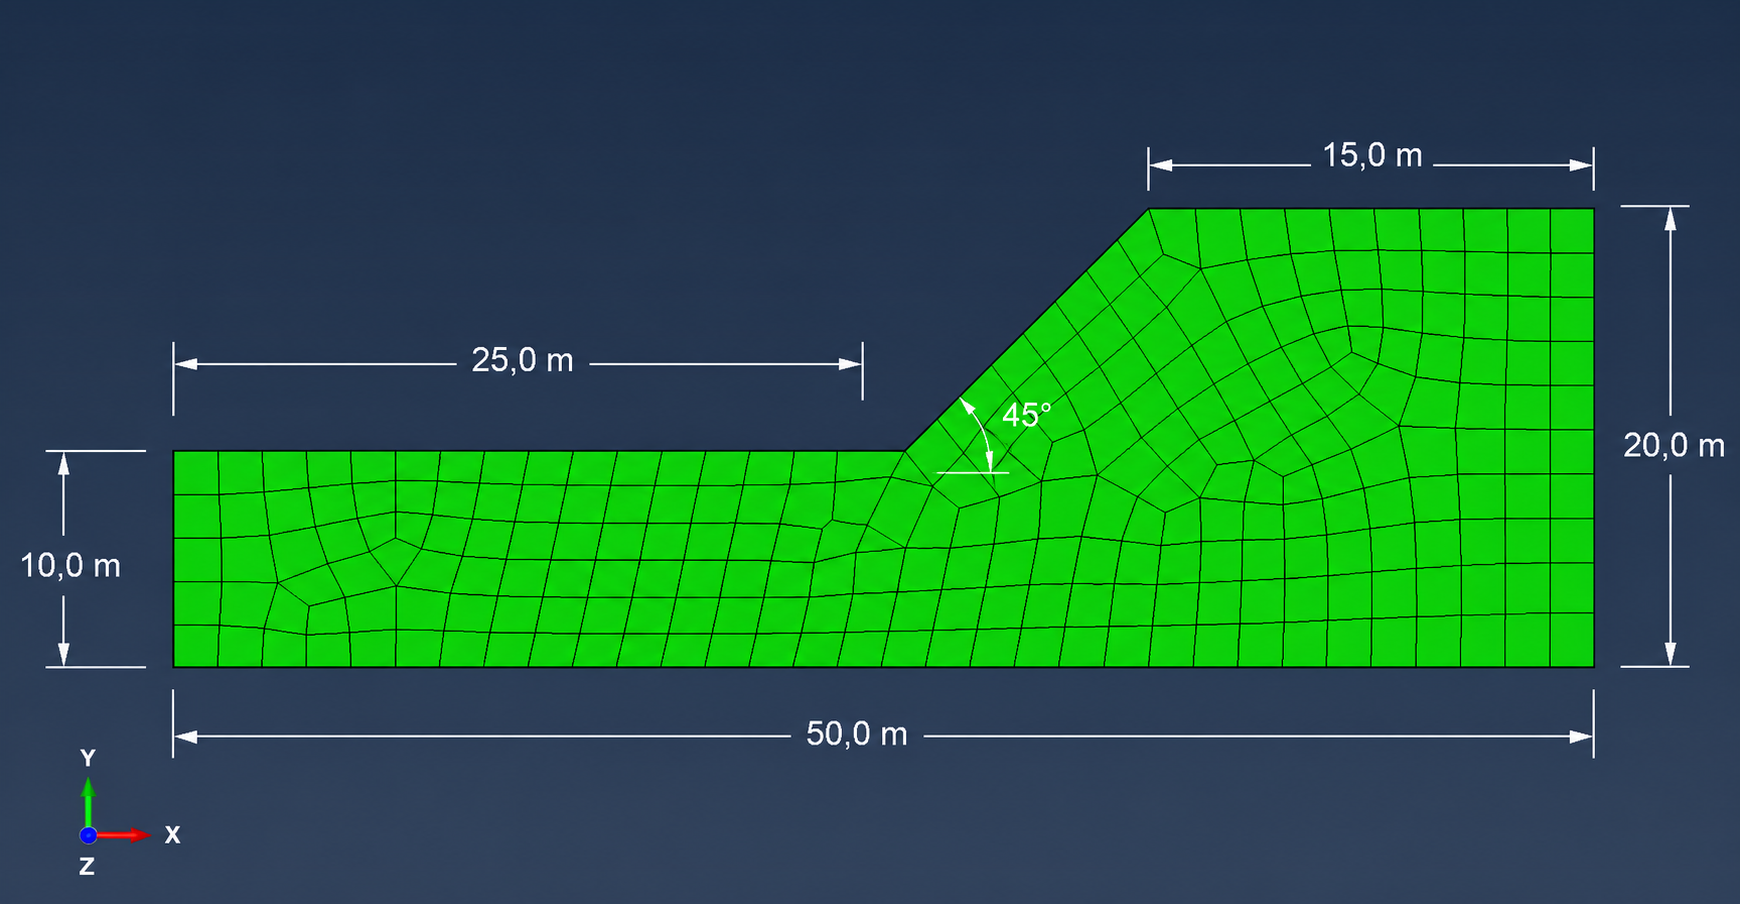
\includegraphics[width=0.9\textwidth]{Figures/talude_referencia.png}
\end{center}
\vspace{6pt}
\begin{center}
\captionof{figure}{Reference model: classical slope (60\,m base, 20\,m height), boundary conditions, and location of investigation point $P$.}
\label{fig:talude_referencia}
\end{center}

% --------------------------------------------------------------------------
\subsection{Investigation Point and Comparison Metric}\label{subsec:ponto_investigacao}
% --------------------------------------------------------------------------

To make the comparison between Abaqus and MPM objective, an investigation point is defined within the slope, corresponding to the same physical region monitored in the ongoing simulations. At this point, the static reference stress is extracted from Abaqus, while in MPM the temporal evolution of the stress component of interest is recorded throughout accommodation.

This strategy enables comparison of two complementary aspects: (i) the asymptotic value reached by each integrator and its distance from the static reference; and (ii) transient response behavior, including oscillation amplitude, damping rate, and possible initial overshoot. Instead of relying only on final stress maps, the analysis explicitly considers the temporal convergence history.

% --------------------------------------------------------------------------
\subsection{Accommodation Stopping Criteria}\label{subsec:criterios}
% --------------------------------------------------------------------------

Two distinct criteria were evaluated to determine when the accommodation phase can be considered complete and to organize interpretation of results at the investigation point.

\noindent \textbf{\textit{Criterion A -- Long-duration run ($t$ large)}}. This follows the usual practice of running the simulation for a sufficiently long time until the system appears stabilized, then evaluating the final state obtained with each integrator. This criterion has relevant limitations: the definition of "long enough" is subjective, may mask residual instabilities not visible by eye, and often implies unnecessary computational cost.

\noindent \textbf{\textit{Criterion B -- Kinetic energy}}. An automatic criterion is proposed in which accommodation is declared complete when the global kinetic energy, $E_k(t)$, drops below a fraction $\varepsilon$ of the maximum value observed during the simulation, i.e., $E_k(t)/E_{k,\text{max}} < \varepsilon$. This criterion is objective and scale-independent, enabling quantitative comparison among integrators in terms of both accommodation time and achieved convergence accuracy.

% --------------------------------------------------------------------------
\section{Results}\label{sec:resultados}
% --------------------------------------------------------------------------

This section presents geostatic-accommodation results for the classical slope obtained with the three integrators (USL, USF, and MUSL), under the two stopping criteria described in Section \ref{subsec:criterios}, in comparison with the Abaqus static reference solution. The main focus is the stress monitored at the investigation point and how each integrator converges over time toward the reference geostatic value.

% --------------------------------------------------------------------------
\subsection{Abaqus Static Reference Stress}\label{subsec:ref_abaqus}
% --------------------------------------------------------------------------

Before comparing integrators, the static stress value obtained in Abaqus at the investigation point is presented, together with the corresponding slope stress field. This value is the reference used to evaluate residual error of each integrator at the end of accommodation.

\vspace{6pt}
\begin{center}
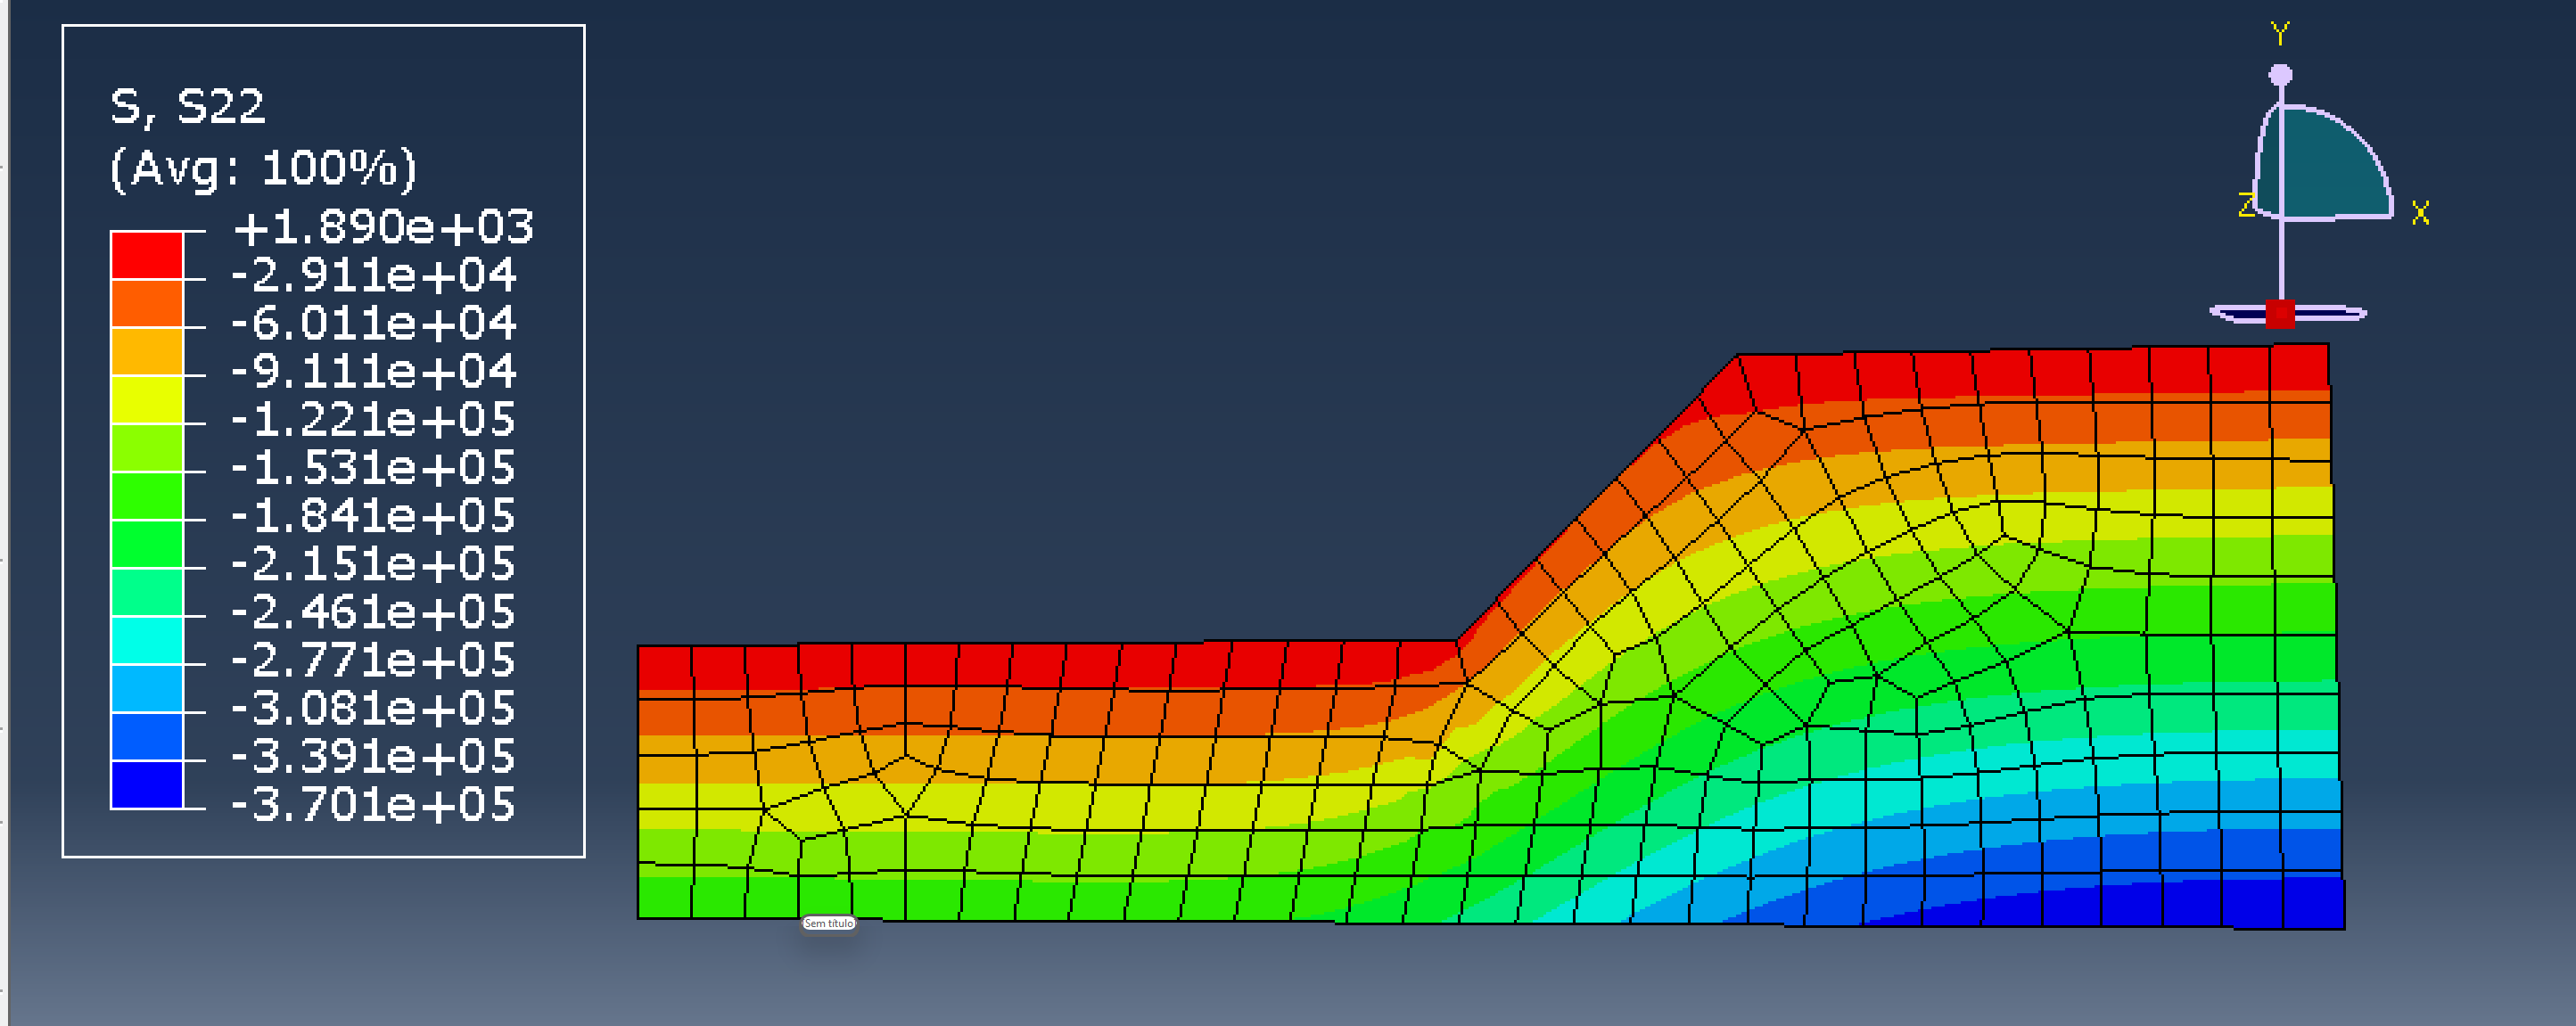
\includegraphics[width=0.9\textwidth]{Figures/abaqus_referencia.png}
\end{center}
\vspace{6pt}
\begin{center}
\captionof{figure}{Abaqus static reference solution: $\sigma_{zz}$ stress field in the slope under geostatic equilibrium.}
\label{fig:abaqus_referencia}
\end{center}

\begin{center}
\begin{tabular}{ccc}
\hline
Investigation point & Monitored component & Abaqus value \\ \hline
to be filled & to be filled & to be filled \\ \hline
\end{tabular}
\end{center}

% --------------------------------------------------------------------------
\subsection{Temporal Stress History at the Investigation Point}\label{subsec:curvas_tensao}
% --------------------------------------------------------------------------

The temporal stress curves at the investigation point allow direct visualization of the accommodation process. Comparison with the Abaqus reference line highlights both convergence rate and the intensity of numerical oscillations produced by each integrator.

\vspace{6pt}
\imagemplaceholder{Temporal stress curves at the investigation point for USL, USF, and MUSL, together with the horizontal line corresponding to the Abaqus static value.}{6cm}
\vspace{6pt}
\begin{center}
\captionof{figure}{Temporal stress evolution at the investigation point: comparison among Abaqus, USL, USF, and MUSL.}
\label{fig:curvas_tensao_ponto}
\end{center}

\begin{center}
\begin{tabular}{lccc}
\hline
Integrator & Final stress & Relative error vs. Abaqus & Observed oscillation \\ \hline
USL & to be filled & to be filled & to be filled \\
USF & to be filled & to be filled & to be filled \\
MUSL & to be filled & to be filled & to be filled \\ \hline
\end{tabular}
\end{center}

% --------------------------------------------------------------------------
\subsection{Convergence and Kinetic Energy}\label{subsec:conv_energia}
% --------------------------------------------------------------------------

In addition to the local stress value, convergence is analyzed through global kinetic energy. Comparing the $E_k(t)$ curves helps identify which integrator dissipates residual energy faster and at what time each solution can be considered sufficiently accommodated.

\vspace{6pt}
\imagemplaceholdermeia{Kinetic-energy curves $E_k(t)$ for USL, USF, and MUSL.}{4cm}
\hfill
\imagemplaceholdermeia{Zoom of the convergence region highlighting the criterion $E_k/E_{k,\max} < \varepsilon$.}{4cm}
\vspace{6pt}
\begin{center}
\captionof{figure}{Comparison of integrator kinetic-energy curves and identification of accommodation time.}
\label{fig:energia_convergencia}
\end{center}

\begin{center}
\begin{tabular}{cccc}
\hline
Integrator & $t_{\text{accommodation}}$ & $\varepsilon$ & Observation \\ \hline
USL & to be filled & to be filled & to be filled \\
USF & to be filled & to be filled & to be filled \\
MUSL & to be filled & to be filled & to be filled \\ \hline
\end{tabular}
\end{center}

% --------------------------------------------------------------------------
\subsection{Consolidated Integrator Comparison}\label{subsec:comparativo}
% --------------------------------------------------------------------------

Table \ref{tab:comparativo} summarizes the consolidated results for the three integrators in terms of final stress at the investigation point, relative error against Abaqus, and time required to reach the accommodation criterion.

\begin{center}
\captionof{table}{Overall integrator comparison -- response at the investigation point and convergence.}
\label{tab:comparativo}
\begin{tabular}{lccccc}
\hline
Integrator & Final stress & Abaqus stress & Relative error & $t_{\text{accommodation}}$ & Observation \\ \hline
USL  & to be filled & to be filled & to be filled & to be filled & to be filled \\
USF  & to be filled & to be filled & to be filled & to be filled & to be filled \\
MUSL & to be filled & to be filled & to be filled & to be filled & to be filled \\ \hline
\end{tabular}
\end{center}

\vspace{8pt}
\noindent \textit{Stress maps at the final accommodation stage -- side-by-side comparison.}

\vspace{6pt}
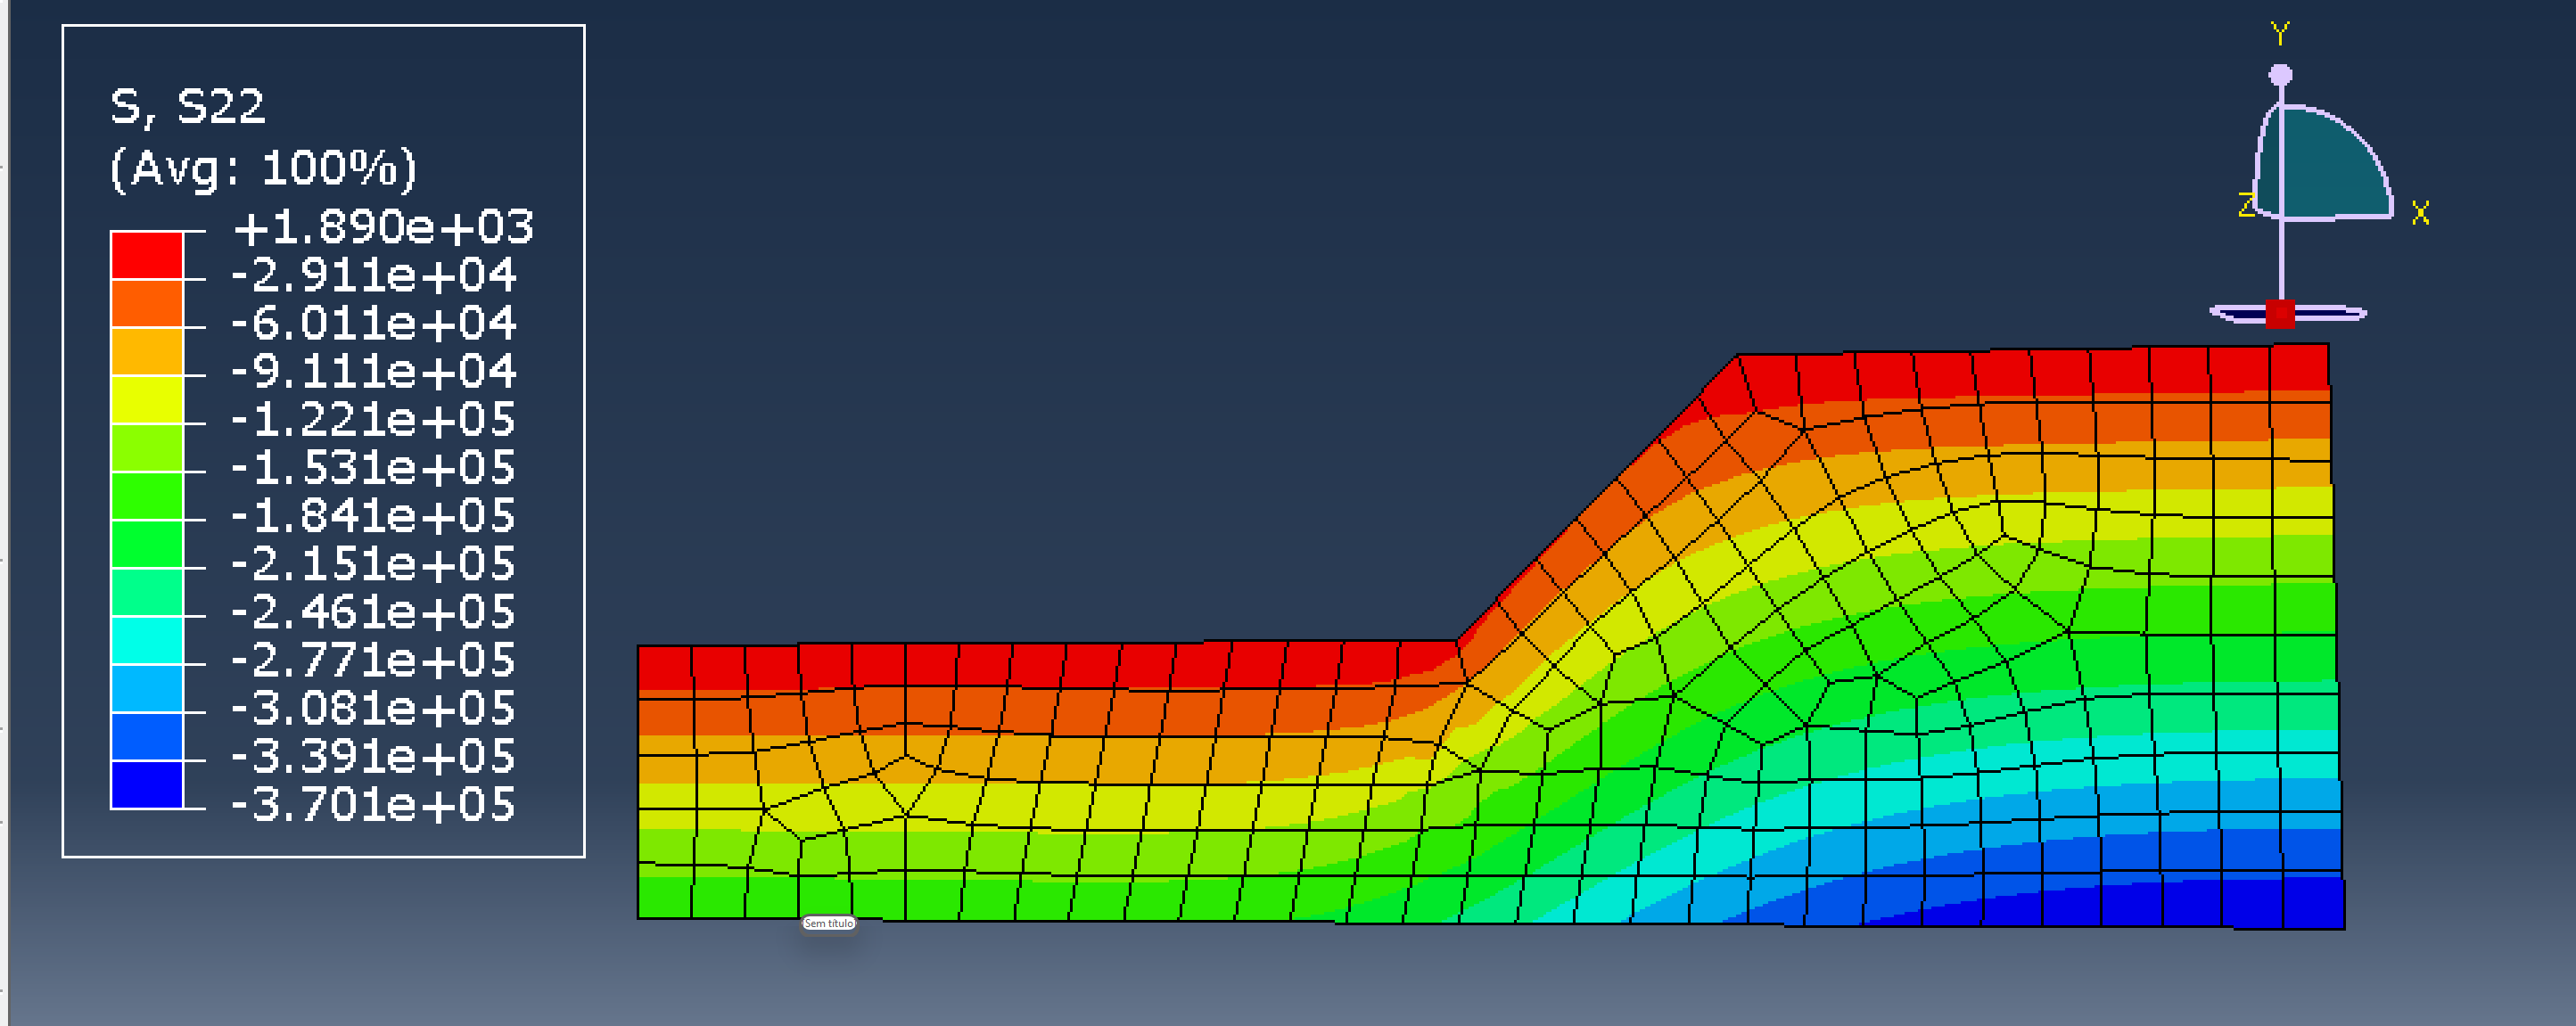
\includegraphics[width=0.46\textwidth]{Figures/abaqus_referencia.png}
\hfill
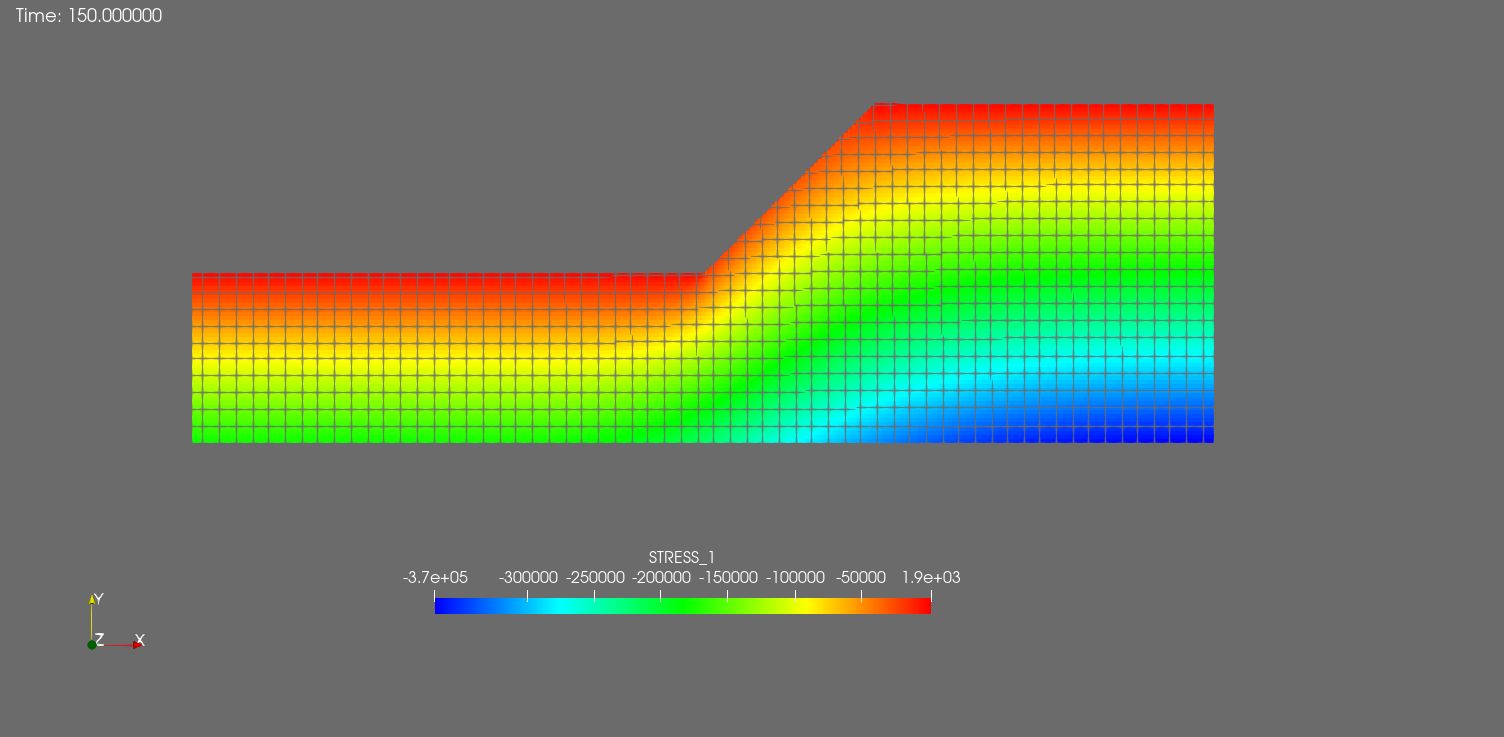
\includegraphics[width=0.46\textwidth]{Figures/USL_Oficial_sta.png}

\vspace{6pt}
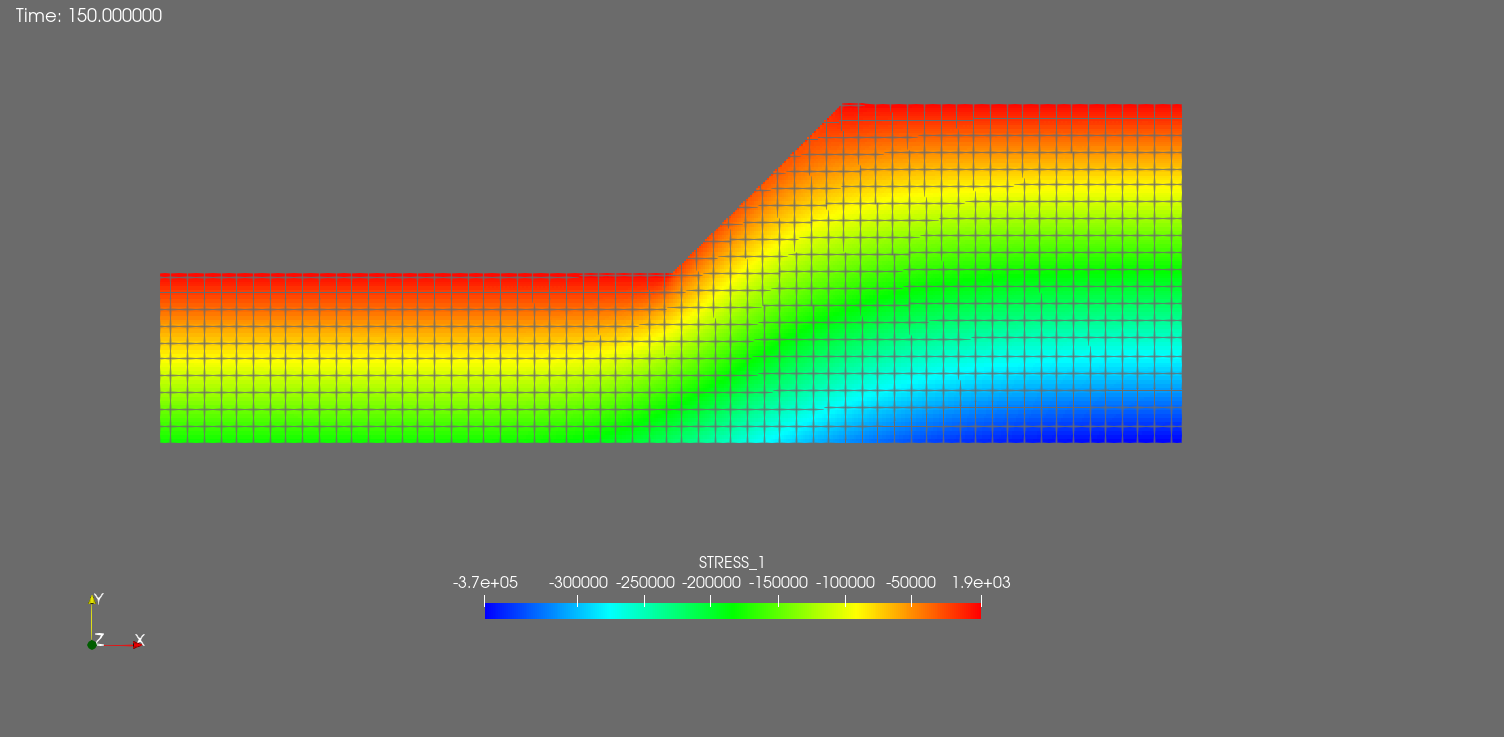
\includegraphics[width=0.46\textwidth]{Figures/USL_Stability.png}
\hfill
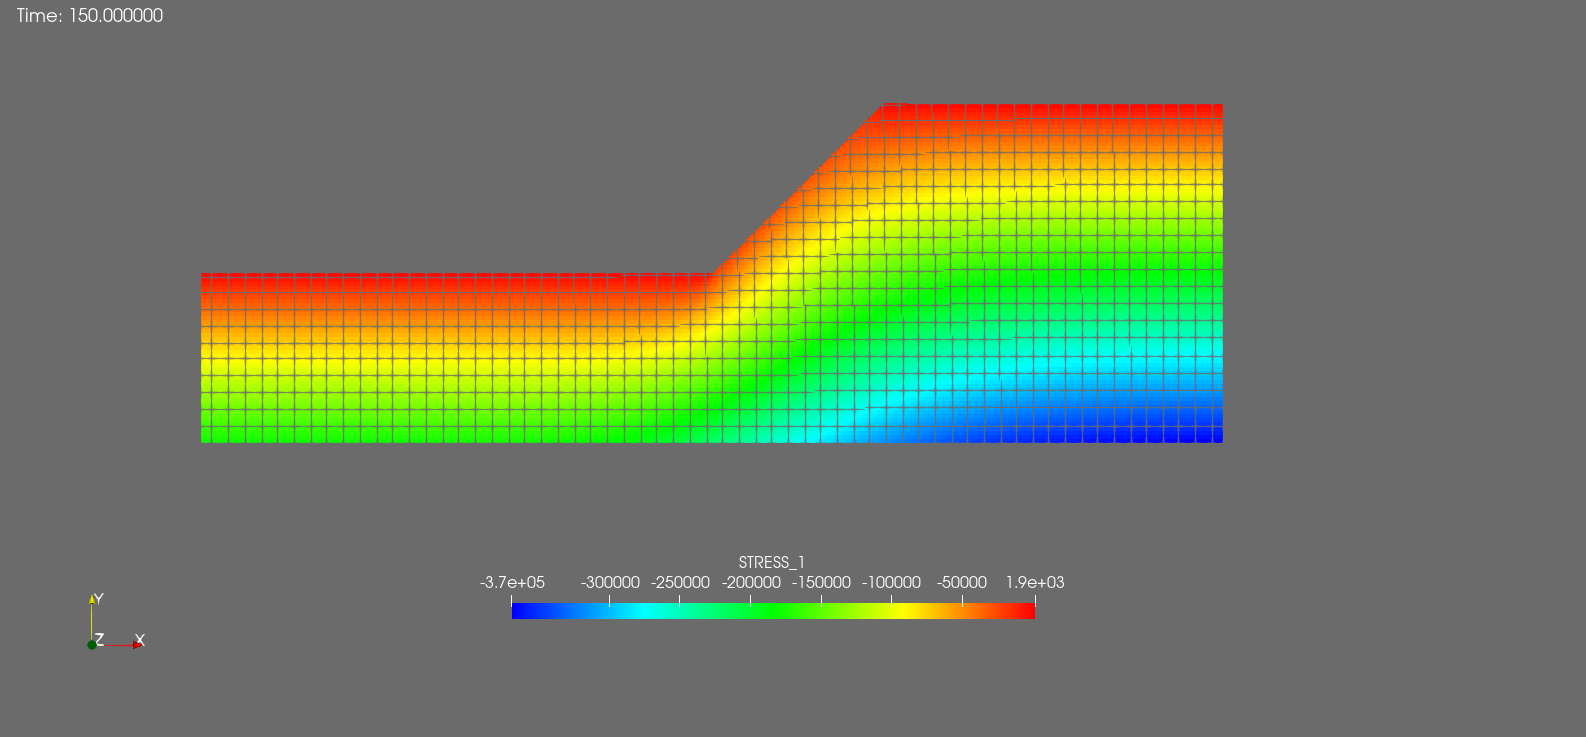
\includegraphics[width=0.46\textwidth]{Figures/MUSL_Stability.png}
\vspace{6pt}
\begin{center}
\captionof{figure}{Side-by-side comparison of final stress maps: Abaqus (reference), USL, USL Stability, and MUSL.}
\label{fig:mapas_comparativos}
\end{center}

\vspace{8pt}
\noindent \textit{Kinetic-energy curves $E_k(t)$.}

\vspace{6pt}
\imagemplaceholder{Overlaid kinetic-energy curves $E_k(t)$ for USL, USF, and MUSL.}{6cm}
\vspace{6pt}
\begin{center}
\captionof{figure}{Comparison of $E_k(t)$ kinetic-energy curves among the three integrators.}
\label{fig:ek_comparativo}
\end{center}

% --------------------------------------------------------------------------
\section{Conclusions and Next Steps}\label{sec:conclusao}
% --------------------------------------------------------------------------

% TODO: fill after consolidation of numerical results.

%-------------------------------------------------------------------------
\vspace{20pt}
\noindent \textbf{Acknowledgements.} [Insert acknowledgements -- e.g., funding agencies, LCCV/UFAL, and E-Sub project collaborators.]
\vspace{12pt}

%--------------------------------------------------------------------------
\noindent \textbf{Authorship statement.} The authors hereby confirm that they are the sole liable persons responsible for the authorship of this work, and that all material that has been herein included as part of the present paper is either the property (and authorship) of the authors, or has the permission of the owners to be included here.

\bibliography{bibliography}

\end{document}